\documentclass[10pt]{report}
\usepackage[left=25mm,right=25mm,top=30mm,bottom=30mm]{geometry}
\usepackage{amsmath} % math
\usepackage{amssymb} % math
\usepackage{graphicx} % to use \includegraphics{}
\usepackage{diagbox} % to make tables
\usepackage[hangul]{kotex}
\usepackage{multirow} % to make tables
\usepackage{caption}
\usepackage[hidelinks]{hyperref}
\usepackage{color}
\newcommand{\std}{\href{http://stdweb2.korean.go.kr}{\color{blue}국립국어원 표준국어대사전}}
\begin{document}
\begin{center}
	\Large 국어와 생활 시험범위 정리
	\normalsize
	\begin{flushright}
		경기과학고등학교 14041 박승원
		
		\today
	\end{flushright}
	이 문서의 차례 및 표 목록은 맨 뒤에 있음. \color{blue}{\#시험기간이라서}
	\begin{figure}[h]
		\begin{center}
			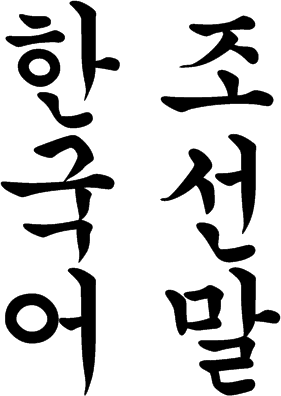
\includegraphics{Korean.png}
			\caption{\href{https://en.wikipedia.org/wiki/Korean_language}{위키백과에 소개된 우리말의 두 가지 명칭.}}
		\end{center}
	\end{figure}
\end{center}
이 문서는 경기과학고등학교에 재직 중이신 이동학 선생님의 `국어와 생활'  수업자료를 바탕으로 만들어졌습니다.

Creative Commons CC BY-NC-SA


%\tableofcontents
\chapter{언어}
\begin{center}
	``언어와 사고는 상호 의존적이다.'' \\
	``언어는 한 사회의 문화를 반영하고, 동시에 한 사회의 문화를 형성한다.''
\end{center}
\section{언어의 특성}
\begin{itemize}
\item 기호성 : 표현하고자 하는 내용을 일정한 형식으로 나타내는 기호
\item 자의성 : 내용\footnote{의미}과 형식\footnote{기호} 사이의 필연성 없음
\item 사회성 : 내용과 형식 사이의 관계는 쓰는 사람들간의 무언의 약속
\item 역사성 : 시간의 흐름에 따라 변함
\item 규칙성 : 이루는 각 요소들은 정해진 규칙에 따라 운용\footnote{무엇을 움직이게 하거나 부리어 씀.}
\item 창조성 : 정해진 규칙 안에서 새로운 단어, 문장 무한히 만들 수 있음.
\item 추상성 : 추상화\footnote{기호(형식)은 유한, 내용(의미)는 무한하기 때문에 기호가 내용을 완벽히 표현 불가} 과정을 거친 개념을 단위로 운용
\item 분절성 : 연속적으로 이루어진 세계를 불연속적으로 나타냄

\end{itemize}
\chapter{음운}
음운은, 
\begin{enumerate}
\item 말의 뜻을 구별해주는 : 물 $\leftrightarrow$ 불 $\leftrightarrow$ 풀
\item \textbf{소리}의
\item 가장 작은 단위
\end{enumerate}
이다.\footnote{음성 : 사람이 의사소통을 위하여 발음기관을 통해서 내는 소리 \\ 음절 : 모음과 자음이 결합되어 이루는 발음의 가장 작은 단위}

\section{음운의 종류 및 특징}
음운의 종류에는 `말' 을 `ㅁ', `ㅏ', `ㄹ' 와 같이 나뉘는 분절음운이 있고 그렇지 않은 비분절음운이 있다.
\subsection{분절음운}
\subsubsection{모음}
\begin{center}
모음 : 발음기관의 장애를 받지 않고 나는 소리. 홀로 발음할 수 있음.
\end{center}

모음에는 단모음과 이중모음이 있으나, 여기에서는 단모음에 대해서만 논하고자 한다.
단모음의 발음에 따른 분류는 표 \ref{vowel_pronun}과 같다.
\begin{table}
\begin{center}
	\begin{tabular}{|c|c|c|c|c|}
		\hline
		혀의 앞뒤 위치 & \multicolumn{2}{|c|}{전설 모음} & \multicolumn{2}{|c|}{후설 모음}\\
		\hline
		\diagbox{혀의 높이}{입술모양} & 평순 & 원순 & 평순 & 원순\\
		\hline
		고 & ㅣ & ㅟ & ㅡ & ㅜ\\
		\hline
		중 & ㅔ & ㅚ & ㅓ & ㅗ\\
		\hline
		저 & ㅐ &    & ㅏ &   \\
		\hline
	\end{tabular} 
	\caption{단모음의 발음에 따른 분류}
	\label{vowel_pronun}
\end{center}
\end{table}

\subsubsection{자음}
\begin{center}
자음 : 발음기관의 어디에선가 \textbf{장애}를 받아 만들어지는 소리. 홀로 발음할 수 없음.
\end{center}

자음의 발음에 따른 분류는 표 \ref{consonant_pronun}과 같다.
여기에서 `파찰' 이란 파열과 마찰을 합한 말이다.

\begin{table}
\begin{center}
	\begin{tabular}{|c|c|c|c|c|c|c|}
		\hline
		\multicolumn{2}{|c|}{\diagbox{조음방법}{조음위치}} & 두 입술 & 윗잇몸, 혀끝 & 센입천장, 혓바닥 & 여린입천장, 혀뒤 & 목청 사이 \\
		\hline
		\multirow{3}{*}{파열음}
		& 예사소리 & ㅂ & ㄷ & & \textbf{ㄱ} & \\
		\cline{3-7}	 
		& 된소리   & ㅃ & ㄸ & & \textbf{ㄲ} & \\
		\cline{3-7}	 
		& 거센소리 & ㅍ & ㅌ & & \textbf{ㅋ} & \\ 
		\hline
		\multirow{3}{*}{파찰음}
		& 예사소리 & & & ㅈ & & \\ 
		\cline{3-7}	 
		& 된소리   & & & ㅉ & & \\ 
		\cline{3-7}	 
		& 거센소리 & & & ㅊ & & \\ 
		\hline
		\multirow{2}{*}{마찰음}
		& 예사소리 & & ㅅ & & &\multirow{2}{*}{ㅎ} \\ 
		\cline{3-6}	 
		& 된소리   & & ㅆ & & & \\ 
		\hline
		\multicolumn{2}{|c|}{비음} & ㅁ & ㄴ & & ㅇ & \\
		\hline
		\multicolumn{2}{|c|}{유음} & & ㄹ & & & \\
		\hline
	\end{tabular}
	\caption{자음의 발음에 따른 분류}
	\label{consonant_pronun}
\end{center}
\end{table}

\subsection{비분절음운}
비분절음운에는 장단, 억양 등이 있다. 끝.

\subsection{국어의 음운론적 특징}
\begin{itemize}
\item 예사소리 / 된소리 / 거센소리의 대립
\item 첫소리에 둘 이상의 `ㄹ', `ㄴ' 소리가 오지 않음
\item 모음조화 현상
\end{itemize}

\section{음운의 변동}
국어의 표기는 어법에 맞도록 쓰는 것이 원칙이기 때문에 실제 발음과는 다를 수 있다. 예를 들면 `꽃' 은 상황에 따라 [꼬ㅊ], [꼰], [꼳]으로 다양하게 발음된다.

이와 같이 어떤 음운이 그 놓이는 환경에 따라 다른 음운으로 바뀌어 소리 나는 현상을 음운 변동이라고 한다. 음운 변동은 크게 교체, 탈락, 첨가, 축약과 같이 4가지로 나뉜다. 다음 두 문장에서 그를 살펴보자.

\begin{center}
	철수는 \textit{국물}\footnote{교체}을 \textit{좋아}\footnote{탈락}한다.
	
	\textit{담요}\footnote{첨가}를 \textit{놓고}\footnote{축약} 나오거라.
\end{center}

\subsection{교체}
어떤 음운이 다른 음운으로 바뀌는 현상.
\subsubsection{끝소리 규칙}
음절 끝에서 발음될 수 있는 자음은 ㄱ,ㄴ,ㄷ,ㄹ,ㅁ,ㅂ,ㅇ\footnote{가느다란물방울} 과 같이 7개뿐이기 때문에 음절이 교체된다. 예시는 표 \ref{end_sound_rule}와 같다.

\begin{table}
\begin{center}
	\begin{tabular}{|c|c|c|c|}
		\hline
		잎 & 끝 & 부엌 & 꽃 \\
		\hline
		[입] & [끋] & [부억] & [꼳] \\
		\hline
	\end{tabular}
	\caption{끝소리 규칙의 예시}
	\label{end_sound_rule}
\end{center}
\end{table}

\subsubsection{된소리되기}
다음 4가지의 경우 \textbf{뒤에서} 예사소리가 된소리로 바뀌는 현상.
\begin{enumerate}
\item 파열음\footnote{ㄱ,ㄷ,ㅂ 외 6개}
\item 한자어
\item 용언의 활용
\item 관형사형 어미 `ㄹ'
\end{enumerate}

\subsubsection{구개음화}
단모음 `ㅣ ' 이나 반모음 `j ' 앞에서 `ㄷ,ㅌ' 이 각각 [ㅈ], [ㅊ]로 바뀌는 현상. 예시는 표 \ref{palatalization}와 같다.

\begin{table}
\begin{center}
	\begin{tabular}{|c|c|}
		\hline
		굳이 & 밭+이 \\
		\hline
		[구지] & [바치] \\
		\hline
	\end{tabular}
	\caption{구개음화의 예시}
	\label{palatalization}
\end{center}
\end{table}

\subsubsection{자음동화}
비/유음 앞에서 비/유음이 아닌 것이 비/유음이 되는 바뀌는 비/유음화. 예시는 표 \ref{consonant_story}와 같다.
\begin{table}
\begin{center}
	\begin{tabular}{|c|c|c|c|c|c|c|}
		\hline
		 & & $\rightarrow$ & & & $\rightarrow$ & \\
		\hline
		\multirow{3}{*}{비음화}
		& ㅂ & & ㅁ & 밥물 & & 밤물\\
		\cline{2-7}
		& ㄷ & & ㄴ & 걷는다 & & 건는다\\
		\cline{2-7}
		& ㄱ & & ㅇ & 국물 & & 궁물\\
		\hline
		유음화 & ㄴ & & ㄹ & 신라 & & 실라\\
		\hline
	\end{tabular}
	\caption{자음동화의 예시}
	\label{consonant_story}
\end{center}
\end{table}

\subsubsection{`ㅣ' 모음 역행동화}
`ㅣ ' 앞에서 `ㅏ ', `ㅓ ' 등의 후설 모음이 전설 모음으로 바뀌는 현상. \footnote{풋내기, 냄비, 멋쟁이는 원래는 표준어가 아닌 표준 발음에 속했으나 현재는 표준어로 인정됨.} 예시는 표 \ref{counter_story}와 같다.

\begin{table}
\begin{center}
	\begin{tabular}{|c|c|c|c|c|}
		\hline
		어미 & 고기 & 멋장이 & 풋나기 & 남비 \\
		\hline
		[에미] & [괴기] & 멋쟁이 & 풋내기 & 냄비\\
		\hline
	\end{tabular}
	\caption{`ㅣ' 모음 역행동화의 예시}
	\label{counter_story}
\end{center}
\end{table}

\subsubsection{교체 문제들}
다음 단어들은 음운의 교체에 해당한다. 분류하시오.
\begin{center}
	부엌, 국밥, 국민, 신라, 굳이, 아기
\end{center}

\subsection{탈락}
있었던 음운이 사라지는 현상.
\subsubsection{자음의 탈락}
\begin{enumerate}
\item 음절 끝에는 하나의 자음밖에 오지 못함 : 몫[목], 닭[닥]
\item 모음 사이에 최대 두개의 자음 : 짧고[짤꼬], 굵고[굴:꼬], 좋은[조은], 날는[나는]
\end{enumerate}

\subsubsection{모음의 탈락}
용언이 활용될 때 어간이나 어미의 모음에서 나타난다. 예시는 표 \ref{vowel_omission}와 같다.

\begin{table}
\begin{center}
	\begin{tabular}{|c|c|c|c|}
		\hline
		쓰-+-어라 & 자-+-아라 & 서-+-어라 & 끄-+-어라 \\
		\hline
		써라 & 자라 & 서라 & 꺼라 \\
		\hline
	\end{tabular}
	\caption{모음의 탈락의 예시}
	\label{vowel_omission}
\end{center}
\end{table}

\subsection{첨가}
없었던 음운이 새로 보태지는 현상.
\subsubsection{ㄴ첨가}
합성어나 파생어 등에서 뒷말이 모음 `ㅣ' 이나 반모음 `j' 로 시작될 때 나타남. 이는 사잇소리 현상\footnote{두개의 형태소 또는 단어가 합쳐져서 합성어(명사)가 될 때, 그 사이에 소리가 덧생기는 현상(ㄴ이 첨가되거나 된소리가 남)}의 하나이다. 예시는 표 \ref{sickle_addition}와 같다.

\begin{table}
\begin{center}
	\begin{tabular}{|c|c|c|c|}
		\hline
		담요 & 솜+이불 & 한+여름 & 맨+입\\
		\hline
		[담뇨] & [솜니불] & [한녀름] & [맨닙]\\
		\hline
	\end{tabular}
	\caption{`ㄴ' 첨가의 예시}
	\label{sickle_addition}
\end{center}
\end{table}

\subsection{축약}
두 음운이 합쳐져 새로운 음운이 되는 현상.
\subsubsection{거센소리되기}
`ㅎ' + 앞뒤의 예사소리 $\rightarrow$ 거센소리

예시는 표 \ref{aspirated}와 같다.
\begin{table}
\begin{center}
	\begin{tabular}{|c|c|c|c|}
		\hline
		입학 & 좋다 & 옳지 & 많다 \\
		\hline
		[이팍] & [조타] & [올치] & [만타] \\ 
		\hline
	\end{tabular}
	\caption{거센소리되기의 예시}
	\label{aspirated}
\end{center}
\end{table}

\chapter{단어}
\section{품사}
품사의 분류 기준은 \textbf{형태, 기능, 의미}이다.
\subsection{용언}
문장에서 서술의 기능을 하는 단어.

형태가 변하는\footnote{활용} 유일한 `언' 이다. 체언, 관계언, 수식언, 독립언은 형태가 변하지 않는다. 단, 예외적으로 활용되는 `-이다' 와 같은 서술격조사가 있긴 함.
\subsubsection{동사}
사람이나 사물의 움직임을 나타내는 단어
\subsubsection{형용사}
사람이나 사물의 성질 혹은 상태를 나타내는 단어
\subsection{체언}
문장에서 몸\textbf{체}가 되는 부분.
\subsubsection{명사}
구체적/추상적인 대상의 이름을 나타내는 단어.
의존명사에 관해서는 \pageref{consonant_pronun}쪽의 \ref{consonant_pronun}절을 참조 바람.
\subsubsection{대명사}
사람이나 장소의 이름을 대신하여 가리키는 단어.
\begin{itemize}
\item 인칭대명사 : 저, 너, 너희, 우리, 자네, 누구
\item 지시대명사 : 거기, 무엇, 그것, 이것, 저기
\end{itemize}
※아버지 : 명사임.
\subsubsection{수사}
순서\footnote{서수사}/수량\footnote{양수사}을 나타내는 수사.
\subsection{관계언}
주로 체언 뒤에 붙어 다양한 문법적 관계를 나타내거나 의미를 추가하는 단어.
\subsubsection{조사}
특수한 의미를 더해 주는 단어들.

\textbf{을/를, 이/가, 은/는, 와/과, 의, 에서, 에게, 이다} 등

\subsection{수식언}
다른 단어를 꾸며 주는 역할을 하는 단어들.

\subsubsection{관형사}
체언 앞에 놓여서 체언을 꾸며 주는 역할을 하는 단어들. \textbf{`어떤'}
\subsubsection{부사}
용언을 꾸며 주는 단어들. \textbf{`어떻게'}

\subsection{독립언}
문장에서 독립적으로 쓰이는 \textbf{감탄사}.
\subsubsection{감탄사}
놀람, 느낌, 부름, 대답 등을 나타내는 단어들.

\section{형태소}
형태소 : 일정한 뜻을 가진 가장 작은 말의 단위. $\neq$단어
\begin{itemize}
\item 자립형태소/의존형태소
\item 실질형태소/형식형태소
\end{itemize}
설명은 표 \ref{morpheme}을 참조\footnote{`참고' 과 `참조' 의 차이점? 이번에도 \std 를 사용!\\ 살펴서 생각함, 살펴서 도움이 될 만한 재료로 삼음 / 참고로 비교하여 대조해 봄} 바람.
\begin{table}
\begin{center}
	하늘이 높다.
		\begin{tabular}{|c|c|c|c|}
			\hline
			하늘 & 이 & 높- & -다 \\
			\hline
			자립 & 의존 & 의존 & 의존 \\
			\hline
			실질 & 형식 & 실질 & 형식 \\
			\hline
		\end{tabular}
	\caption{형태소 분석의 예}
	\label{morpheme}
\end{center}
\end{table}

\section{어간/어미, 어근/접사}
\begin{itemize}
\item 어간 : \textbf{용언}이 활용될 때 변하지 않는 부분
\item 어미 : 어간 뒤에 붙어서 변하는 부분
\end{itemize}

기본형을 써보고 비교하면 어간을 찾을 수 있다. 

\begin{center}
	\underline{도착하}시었겠구나.
	
	기본형 : \underline{도착하}다
\end{center}
\begin{itemize}
\item 어근 : 단어를 형성할 때 실질적인 의미를 나타내는 중심 부분
\item 접사 : 어근에 붙어 그 뜻을 제한하거나 품사를 바꾸는 주변 부분
\end{itemize}

\section{단어의 형성}
\subsection{단일어}
단일어 : 어근 하나로 이루어진 단어

\subsection{복합어}
복합어 : 둘 이상의 어근이나 어근과 접사로 이루어진 단어

\subsubsection{합성어}
합성어 : 둘 이상의 어근이 결합한 단어

\subsubsection{파생어}
파생어 : 어근과 접사가 결합한 단어.
\begin{center}
	개-살구, 먹-이다, 먹-구름, 먹-이
\end{center}
복합어는 가끔 보면 합성어인지 파생어인지 구별이 잘 안될 때가 있다. 한 가지 구별 방법은, 합성어는 거의 \textbf{대등}한 두 단어가 사용된다는 것이다.
잘 모르겠으면 역시 \std 에서 찾아보자!

\chapter{문장}
문장 : 우리의 생각이나 감정을 완결된 내용으로 표현하는 최소의 언어 형식
\section{문장성분}
문장성분 : 문장을 만드는 데 일정한 문법적 기능을 하는 부분. 큰 갈래/작은 갈래로 총 3/7가지로 분류됨.
\subsection{주성분}
문장구성의 필수 성분.
\subsubsection{주어}
동작 상태의 주체를 표현.
\subsubsection{서술어}
주어의 동작, 상태, 성질 따위를 풀이.
\subsubsection{목적어}
서술어의 동작 대상을 표현.
\subsubsection{보어}
`되다', `아니다' 가 필요로 하는 주어를 제외한 성분.
\subsection{부속성분}
주성분을 꾸며주는 성분.
\subsubsection{관형어}
체언을 꾸며줌.
\subsubsection{부사어}
체언이 아닌 것들을 꾸며줌.
\begin{center}
	그는 아주\footnote{부사어} 새\footnote{관형어} 사람이\footnote{보어} 되었다.
\end{center}
\subsection{독립성분 - 독립어}
말그대로 어떠한 다른 문장 성분과도 관계를 맺지 않는다. 독립언과 같다고 생각할 수 있지만 꼭 그렇지는 않다.
\begin{itemize}
\item \underline{철수야}, 여기 앉아.
\item \underline{청춘}, 이것은 듣기만 해도 가슴이 설레는 말이다.
\item \underline{어머}, 놀랐잖아.
\item \underline{예}, 맞습니다.
\item 날씨가 흐리다. \underline{그러나} 비는 오지 않았다.
\end{itemize}
\section{문장성분에 관한 몇가지 첨언}
\subsection{서술어의 자릿수}
서술어가 필요로 하는 문장성분의 개수.
\begin{itemize}
\item 한 자리 서술어 : 아름답다, 흐르다, 내리다, 돌아오다, 웃다 등
\item 두 자리 서술어 : 아니다, 던지다, 먹다, 보다, 되다 등
\item 세 자리 서술어 : 주다, 삼다 등
\end{itemize}
\subsection{문장성분을 분석하기 위한 요령}
주의 : 요령은 요령일 뿐, 정석은 아님.
\begin{itemize}
\item 헷갈릴 경우 일단 서술어의 개수를 세어 보아라. 서술어로 쓰이는 품사들에는 동사, 형용사, 그리고 서술격조사 `이다'  뿐이다.
\item \color{blue}{추가바람}
\end{itemize}
\section{홑문장}
주어-서술어 관계가 한 번만 있는 문장. 단순.
\section{겹문장}
주어-서술어 관계가 두 번 이상 있는 문장. 이는 이어진문장과 안은문장으로 나뉜다.
\subsection{이어진문장}
이어진문장 : 두 문장이 서로 나란히 이어져 만들어진 겹문장.
\subsubsection{대등}
독립, 나열

-고, -지만, -으나, -으며
\subsubsection{종속}
배경, 조건, 원인, 의도, 양보...

-는데, -으면, -아서,-으려고, -을지라도
\subsection{안은문장과 안긴문장}
안은문장 : 한 문장이 다른 문장을 안아 만들어진 겹문장. 여기에서 `안긴'  문장을 안긴문장이라 한다.
\begin{itemize}
\item 명사절 : -음, -기
\item 관형절 : -은, -는, -던, -을
\item 부사절 : -이, -게, -도록
\item 서술절 : 이중주어문
\item 인용절 : -라고, -하고, -고
\end{itemize}
\section{비문 분석}
\begin{center}
	비문(非文) : 문법에 맞지 않는 문장.
	\begin{flushright}
		\small -국립국어원 표준국어대사전
	\end{flushright}
\end{center}
비문의 종류는 다음과 같이 매우 다양하다. 11시 59분에 제출된 숙제에서 많이 볼 수 있다는...
\begin{itemize}
\item 주술 호응이 이루어지지 못한 경우.

\item 구조어의 호응이 이루어지지 못한 경우.

\item 높임법의 호응이 이루어지지 못한 경우.\footnote{`있다 ' 의 직접높임말로는 `계시다', 간접높임말로는 `있으시다'  가 있다.}

\item 인용법에서 잘못된 조사의 사용.

\item 문장 접속 시 조응이 부적절한 경우.

\item 문장 접속 시 논리적 호응이 이루어지지 못한 경우.

\item 서술어의 어색한 사용(외국어식 표현).\footnote{시간의 흐름에 따라 신세대는 어색함을 느끼지 못하게 되고, 언어의 역사성이 말해주듯 `약속'  이 바뀌게 되는 경우도 있다.}

\item 피동문의 과용. \textbf{-지다}

\item 어순의 배열이 어색한 경우.

\item 동어의 반복 사용. \textbf{와, 과}

\item 중의적 문장(의미의 모호성).

\end{itemize}
\chapter{부록}
\section{의존명사와 띄어쓰기}\label{dependent_noun}
문장에서 홀로 쓰이지 못하고 다른 말에 기대어 쓰이는 명사.
\begin{center}
	아는 대로\footnote{용언 뒤에 붙어있으니 의존명사. 의존명사는 띄어씀.}
	
	너대로\footnote{체언 뒤에 붙어있으니 조사. 조사는 붙여씀.}
\end{center}
\section{사이시옷 현상}
사이시옷 현상은 발음에서의 현상이 아니라 표기상의 문제이므로 부록에 분류하였다. 설명은 표 \ref{between}와 같다.
\begin{table}
\begin{center}
	\begin{tabular}{|c|c|c|}
		\hline
		\multicolumn{2}{|c|}{사이시옷 현상 여부} & \\
		\hline
		순우리말 + 순우리말 & O & 나무+가지, 내+가, 바다+가 \\
		\hline
		순우리말 + \textit{한자어} & O & 터+\textit{세}, \textit{장미}+빛, \textit{등교}+길, \textit{최대}+값 \\
		\hline
		\textit{한자어} + \textit{한자어} & X & \small{예외} \\
		\hline
	\end{tabular}
	\caption{사이시옷 현상의 예시}
	\label{between}
\end{center}
\end{table}
\textit{한자어} + \textit{한자어}의 예외 : 곳간, 찻간, 셋방, 숫자, 툇간, 횟수

\section{비문들}
\begin{itemize}
\item
맑은 물과 흰구름이 감도는 봉우리를 바라보며 우리는 한 걸음 한 걸음 비경으로 들어갔다. 

\item
나는 훔볼트의 언어는 유한한 수단을 무한하게 부려 쓰는 것이라는 언어관에 공감하고 있다. 

\item
영수는 열심히 공부를 학교에서 한다. 

\item
그의 나에 대한 평가는 참으로 어떠한지 궁금하다. 

\item
나는 벌써 어른이 아니면서 앞당겨서 어른의 세계에 물들고 있는 것은 아닐까?

\item
미리 자료를 예비한 분은 별도의 자료를 따로 만들 필요가 없습니다.

\item
담징의 작품은 관념의 표백에 그쳤을는지도 알 수 없다. 

\item
그는, 하겠다고 말한 것은 결코 해내는 사람이다. 

\item
이런 무료한 시간에 그런 회상의 유혹을 물리치기란 좀처럼 어려운 일이었다. 

\item
이들은 비단 조선 시대의 화풍에 반기를 들고, 풍속화를 대담하게 그렸다. 

\item
우리가 한글과 세계의 여러 문자들을 비교해 볼 때, 매우 조직적이며 과학적이고 독창적인 문자라고 하는 사실은 널리 알려져 있다. 

\item
영수는 은희에게 가방을 주었는데, 그 보답으로 영수에게 책을 선물하였다. 

\item 
우리가 패배한 이유는 상대를 너무 업신여겼다.
\item
나는 너보다 낚시를 더 좋아한다. 

\item
사람은 모름지기 분별을 가질 따름이다. 

\item
그다지 인심이 후하던 그도 세대의 변화에 따라 마음이 달라졌다. 

\item
선생님께 돌 지난 손자가 계시지? 

\item
할아버지께서는 이빨이 좋으시다. 

\item
철수야, 너 아버지께서 오시라고 한다. 

\item
할아버지, 작은아버지께서 오셨습니다.

\item
삼촌은 나만 보면 “너는 커서 뭐가 되고 싶니?”고 묻곤 하셨다.

\item
순희가 자기집 바둑이가 새끼를 여러 마리 낳았다라고 나에게 말했다.

\item
기재 사항의 정정 또는 금융 기관의 수납인 및 취급자인이 없으면 무효입니다

\item
재일 동포들은, 일본 사회의 구성원으로서 모든 의무를 다하고 있으면서도 차별과 합당한 대우를 받지 못하고 있다.

\item
인간은 자연을 지배하기도 하고 복종하기도 한다.

\item
그가 게임에 몰두하는 것은 단순히 즐기기 위해서보다는 현재의 괴로움을 잠시나마 잊어 보려는 행동에 불과하다. 

\item
누나는 모범생이며, 형은 냉면을 좋아한다. 

\item
나는 축구를 좋아하고, 누나의 취미는 탁구이다. 

\item
복남이는 낚시질을 별로 즐기지 않았고, 고기가 입질도 할 낌새가 전혀 안 보였다. 

\item
오는 토요일 설악산으로 여행 갈 계획을 가지고 있습니다. 

\item
너의 행동은 아무리 생각해 보아도 나에게는 이해가 가지를 않는다.

\item
그 사람은 참 훌륭하다고 생각이 듭니다.

\item
이러한 성격 때문에 당해지는 손해가 여간 크지 않았다. 
\item
한 나라의 영화 정책은 당연히 자기 나라 영화의 보호와 진흥을 목적으로 그 방향에 따라 정책을 수행한다.

\item
여기서 알아야 할 점은 일제의 식민지 교육이 식민지 지배의 도구에 지나지 않았으며, 간교한 민족 분열의 수단인 동시에 정치 선전이었다. 

\item
그러나 다행스러운 것은, 그의 불타는 창작 의욕이 그를 죽음에서 구해 내었으며, 인류를 위해 훌륭히 예술을 창작할 것을 결심했던 것이다. 

\item
내가 사랑하는 영희의 언니 영자

\item
선생님이 보고 싶은 학생이 매우 많다. 

\item
그 소설가는 순수한 마음을 가진 어린이와 철학자를 작품의 주인공으로 삼고 있다. 
\item
그것이 요즈음 학생들에게 많이 읽혀지는 책이다.

\item
우리 나라는 그동안 많은 다목적 댐들이 만들어지고, 한강뿐만 아니라 전국의 주요 홍수 통제 시스템들이 마련되어 가고 있다. 
\item
사람들이 많은 도시를 다녀보면 재미있는 일이 많을 것이다.

\item
싱싱한 물고기는 물 속에서 헤엄칠 때만 그 싱싱한 물고기의 은빛 지느러미가 빛난다. 

\item
청소년 담배 흡연율을 줄이기 위해 학교에서는 담배 금연 교육을 실시해야 한다. 

\item
텔레비전의 심야 오락 프로그램은 간혹 지나치게 선정적이고 성적 자극을 유도하는 장면이 있다. 

\item
돌이켜 회고해 보건대 고난의 가시밭길을 우리는 걸어 왔습니다. 

\item
인심이 야박해져서 조그만 일에도 재빨리 이해 타산을 계산하는 요즘 세상이 서글프다.

\item
우리는 살아가는 삶의 방식이 제각기 다르게 살고 있다.

\item
이 때 한 용감한 시민이 소리를 지르면서 도망가는 범인을 뒤쫓기 시작했다. 

\item
내일 아침이면 또 마음이 변해지겠구나.

\item
나도 그렇게 생각되어지더라. 

\item
싸늘하게 식어지면서 굳어가던 그 시체는 내게 큰 충격이었다.

\item
그러나 이상의 문제들이 지금껏 민주적 방법으로 해결되어지지 못했기 때문에 갈등과 불만이 싹텄다.

\item
풍년 농사를 위한 저수지가 관리 소홀과 무관심으로 올 농사를 망쳐 버렸습니다.

\item
내가 말하고 싶은 것은 겨울에 체력 훈련을 열심히 하여야 지난해와 같은 성적을 올릴 수 있을 것이다.

\item
우리들의 의견은 앞으로 농촌 보건 문제에 관심을 갖자는 데 뜻을 모았다.

\item
회장님의 말씀이 계시겠습니다.

\item
컴퓨터를 구매하시면 저희 회사가 직접 교육시켜 드립니다.

\item
이 같은 국내 영어 캠프는 무분별한 학생들의 해외 연수를 줄일 것입니다.

\item
손에 들려져 있어야 할 물건이 보이지 않았다.

\item
열려져 있는 창문으로 모기가 들어왔네.

\end{itemize}

\addcontentsline{toc}{section}{이 문서의 차례 및 표 목록}
\tableofcontents
\listoftables
\end{document}